\section{Editor, Visualization, and Playback}\label{sec:editor-visualization}

The studio surfaces are designed so writing, checking, seeing, and hearing a composition stay in one workspace.
This section documents each user-facing surface in the client application.

\subsection{Monaco editor and diagnostics}\label{subsec:monaco-editor}

The editor pane wraps Monaco with a Motivo-specific language registration.
A Monarch tokenizer highlights statement keywords (\texttt{track}, \texttt{pattern}, \texttt{play}, \texttt{for},
\texttt{if}, \texttt{loop}, etc.), explicit type keywords (\texttt{int}, \texttt{double}, \texttt{bool},
\texttt{note}, \texttt{seq}, \texttt{chord}), instrument names, drum note literals, pitch literals, comments, and
operators.
Two editor themes (light and dark) align with the application chrome.

Completion providers suggest instruments, drum notes, type keywords, common pitch literals (e.g.\ \texttt{C4}),
and snippets for recurring constructs such as new \texttt{track} blocks and \texttt{pattern} declarations.
The editor exposes imperative hooks used by the IDE layer: read and replace buffer text, clear error markers, set a
single error marker with message, and jump the viewport to a line/column.

The \textbf{diagnostics feedback loop} closes on every compile.
When the server returns structured errors, the client maps each diagnostic to Monaco markers (severity, message,
optional range) and focuses the first error.
A logs panel lists the same messages with timestamps; clicking a log entry jumps the editor to that location.
Successful compiles clear markers and blur the editor so attention shifts to the visualizer.

\subsection{Workspace layout and IDE chrome}\label{subsec:ide-workspace}

The workspace shell composes the main panes: header (branding, theme toggle, auth entry), resizable editor column,
visualizer column (piano roll plus playback bar), and collapsible diagnostics/logs strip.
An auth wrapper gates the file explorer and account actions while still allowing anonymous compile-from-scratch.

Keyboard shortcuts wired in the IDE layer include: \textbf{Ctrl/Cmd+S} manual save, compile shortcut, playback transport
shortcut, and a shortcut to focus the logs panel.
Figure~\ref{fig:studio-success-screenshot} shows the assembled workspace after a successful compile.

\subsection{Documents, examples, and persistence}\label{subsec:files-persistence}

\topic{Scratch document.} Every session starts from an in-memory buffer with the default Motivo snippet; it compiles
without login and is lost on full reload unless copied out.

\topic{Example library.} Bundled demonstration compositions open as read-only tabs; guests can compile and play them but
cannot persist edits to the database.

\topic{User files (authenticated).} The file explorer lists PostgreSQL-backed documents.
Users create files, open multiple tabs, rename via patch, delete, and download raw source.
The file workspace tracks dirty state per user-owned document and persists the active tab via
\texttt{PATCH /api/files/:id} on explicit save (toolbar button or Ctrl/Cmd+S).
Tab close prompts to save when the document is dirty.
Only user-owned documents persist; examples and scratch buffers skip server storage.

\subsection{Piano roll visualization}\label{subsec:piano-roll}

MIDI is symbolic: a successful compile yields event data, not audio.
\texttt{parse-midi} converts bytes into note structures; \texttt{PianoRoll} renders colored rectangles as
absolutely-positioned DOM elements (CSS layers) with a vertical pitch axis (piano-style) and horizontal time.
Hooks track note range for scaling and playhead position during playback so the scroll view stays aligned with heard
time.

\subsection{Playback and download}\label{subsec:playback}

Playback uses Tone.js with SoundFont-loaded General MIDI instruments.
\texttt{flatten-midi-notes} prepares schedulable events; drum tracks map through a dedicated drum note map.
\texttt{PlaybackBar} exposes play, stop, progress scrubbing, and \textbf{download MIDI} (client-side blob save of the
last successful compile).
Audio runs entirely in the browser; the server never streams PCM.

\begin{figure}[p]
  \centering
  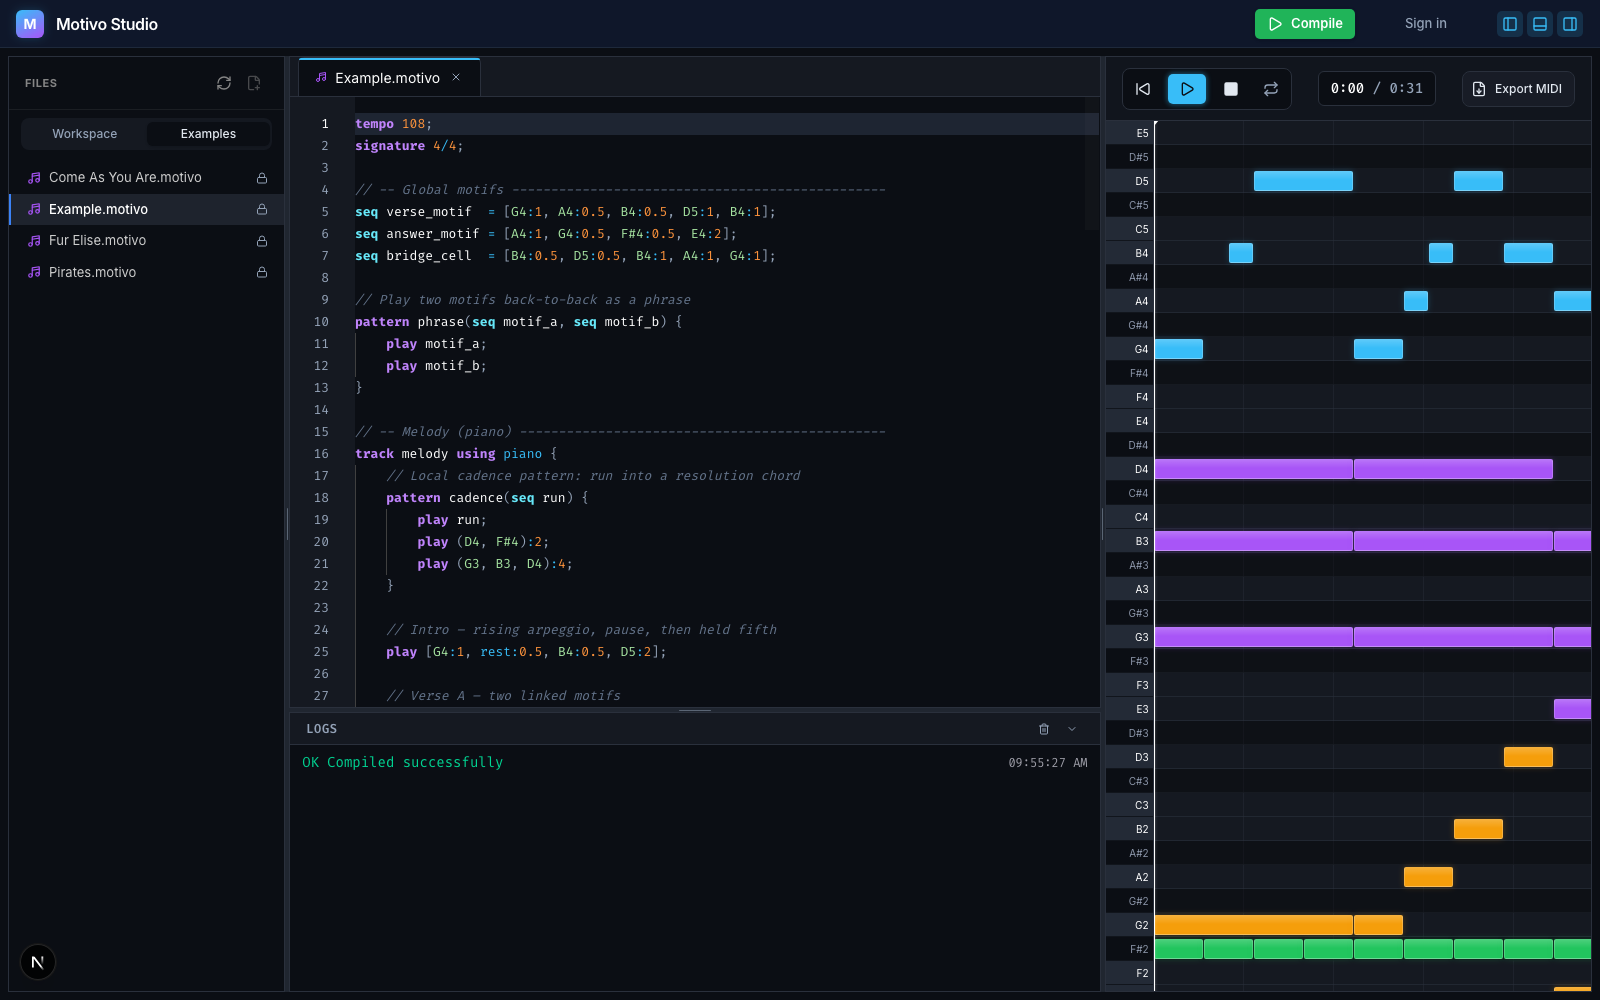
\includegraphics[width=\textwidth]{assets/screenshots/motivo-studio-success.png}
  \caption{Motivo Studio after a successful local compile: Monaco editor, success log, playback controls, and
  piano-roll visualization.}\label{fig:studio-success-screenshot}
\end{figure}

Together, editor diagnostics, file persistence, piano-roll inspection, and SoundFont playback make the studio a
complete development surface for the compiler rather than a thin demo page.
